\documentclass[11pt]{article}
\usepackage{amsmath,amsfonts,amsthm,amssymb}
\usepackage{times}
\usepackage[pdftex]{graphicx}
\usepackage[pdftex,
        colorlinks=true,
        urlcolor=linkblue,     % \href{...}{...} external (URL)
        citecolor=linkred,     % citation number colors
        linkcolor=linknavy,    % \ref{...} and \pageref{...}
        pdftitle={Flame Spread},
        pdfauthor={Andrew Kurzawski},
        pdfsubject={Flame Spread},
        pdfkeywords={UT},
        pdfproducer={pdflatex},
        pagebackref,
        pdfpagemode=UseNone,
        bookmarksopen=true,
        plainpages=false]{hyperref}
\usepackage{pdfsync}
\usepackage{color}
\usepackage{titling}
\usepackage[nottoc,notlof,notlot]{tocbibind} % Put the bibliography and index in the ToC
\usepackage{listings}

\definecolor{linknavy}{rgb}{0,0,0.50196}
\definecolor{linkred}{rgb}{1,0,0}
\definecolor{linkblue}{rgb}{0,0,1}

\setlength{\droptitle}{-4em}     % Eliminate the default vertical space on the title page.
\addtolength{\droptitle}{5cm}   % Only a guess. Use this for adjustment of the title placement.

\setlength{\textwidth}{6.5in}
\setlength{\textheight}{9.0in}
\setlength{\topmargin}{0.in}
\setlength{\headheight}{0.in}
\setlength{\headsep}{0.in}
\setlength{\parindent}{0.25in}
\setlength{\oddsidemargin}{0.0in}
\setlength{\evensidemargin}{0.0in}

% Python Setup
\lstset{
  language=Python,                % choose the language of the code
  basicstyle=\footnotesize,       % the size of the fonts that are used for the code
  numbers=left,                   % where to put the line-numbers
  numberstyle=\footnotesize,      % the size of the fonts that are used for the line-numbers
  stepnumber=1,                   % the step between two line-numbers. If it is 1 each line will be numbered
  numbersep=5pt,                  % how far the line-numbers are from the code
  backgroundcolor=\color{white},  % choose the background color. You must add \usepackage{color}
  showspaces=false,               % show spaces adding particular underscores
  showstringspaces=false,         % underline spaces within strings
  showtabs=false,                 % show tabs within strings adding particular underscores
  frame=single,           % adds a frame around the code
  tabsize=2,          % sets default tabsize to 2 spaces
  captionpos=b,           % sets the caption-position to bottom
  breaklines=true,        % sets automatic line breaking
  breakatwhitespace=false,    % sets if automatic breaks should only happen at whitespace
  escapeinside={\%*}{*)}          % if you want to add a comment within your code
}

% Uncomment lines and make changes to have a header
\newcommand{\code}[1]{ % change to [2]
  % \hrulefill
  % \subsection*{#1}
  \lstinputlisting{#1} % change to {#2}
  \vspace{2em}
}

\title{Quantifying Flame Spread Rate Uncertainty Using Bayesian Methods}
\author{
        \\
        Andrew Kurzawski \\
        Bayesian Statistical Methods \\ 
        Semester Project \\
}
\date{May 3, 2013}

\begin{document}

\maketitle

\clearpage

\pagestyle{plain}


\section{Introduction and Background}

Modeling physical systems requires that we prescribe values for the model parameters based on previous knowledge, correlations, engineering estimations, etc. If we possess expermental data for the system of interest, we can numerically invert for the unknown model parameters. In higher order systems, the solution space may be complicated, and inversion methods can easily get stuck in local minima and maxima. The result of the inversion process is a set of point estimates for the model input parameters. However, it lacks the uncertainty information necessary for activities such as assessing the model's accuracy or conduction a risk assessment.

Bayesian inference offers a means to fit models of physical systems to observed data and calculate the uncertainty in the model parameters. This method assumes that we do not know the true distribution of the input parameters, but we can use observed data to reconstruct it. Given a scenario or collection of scenarios with observed data, Bayesian methods allow us to sample from the true distributions of the data and unobserved quantities of interest (QoI, plural QoIs).

Prediction of fire spread is a major concern to wildland fire fighters who use this information construct tactical plans for supressing and controlling fires. This involves the allocation of resources (personal, command stations, airtankers, etc.) at the appropriate time and location in situations where a poor prediction could cause property damage and put fire figheres and residents lives at risk.

Research efforts in wildland fire modeling have produced models for fire behaviour that range in complexity from algebraic equations to full fluid dynamics and combustion models. This project will focus on the Rothermal flame spread model (ref) that was derived from a combination of fire experiment correlations and physical principles. The result is a set of algebraic equations with eleven input parameters that can be computed quickly. The tradional approach to using the Rothermal model is calculating the flame spread rate using prescribed input parameters based on the fuel type, wind speed, and ground slope. Using this model with Bayesian methods is equivocal to conducting a Bayesian regression where the regression parameters each have a physical meaning, and can therefore be easily examined for non-physical predictions.

The scenario used for this study involves a large scale (~30 acres) field burn conducted at Camp Swift near Bastrop in the Spring of 2011 before Texas saw one of the worst fire seasons on record. The field was composed mostly of Little Bluestem grass with pockets of other vegetation interspersed throughout. We instrumented the field with twenty data loggers to track flame spread and temperature. Flame spread rate in the downwind direction was calculated by the time it took the flame to travel from one data logger to the next divided by the distance. Additionally, data was collected on the moisture content of the grass and weather conditions such as ambient temperature, wind speed and direction, and relative humidity. Some of these values correspond to Rothermal model inputs and will be used as scenario parameters when estimating the likelihood of the observed flame spread rates.


\section{Flame Spread Model Overview}

The Rothermal Model is a system of equations with eleven input parameters that can be used to calculate flame spread rate. Some of these parameters can be measured in the field and others are often prescribed fixed values based on the fuel type (i.e. trees, brush, grass). See Appendix A for descriptions of the input parameters. The full equation for rate of spread, $R$, is as follows:

\begin{equation}
R = \frac{I_R\xi(1+\phi_W+\phi_S)}{\rho_b\epsilon Q_{ig}}
\label{eq:roth_main}
\end{equation}

Each variable in Equation~\ref{eq:roth_main} is a function of one or more other variables that may or may not be input parameters. To make this model more useable, we will simplify the equation in terms of the input parameters. The variables $\xi$, $\rho_b$, and $\epsilon$ are all constructs with limited physical meaning that are each a function of the fuel load ($w_O$), fuel depth ($\delta$), fuel density ($\rho_p$), and surface area to volume ratio ($\sigma$). 

\begin{equation}
\frac{\xi}{\rho_b\epsilon} = \hat{F}(w_O, \delta, \rho_p, \sigma)
\label{eq:roth_fun}
\end{equation}

\noindent where $\hat{F}$ is a combination of polynomial functions of the input parameters which reduces Equation~\ref{eq:roth_main} down to

\begin{equation}
R = \hat{F}(w_O, \delta, \rho_p, \sigma) I_R\frac{1+\phi_W+\phi_S}{Q_{ig}}
\label{eq:roth_fun2}
\end{equation}

$I_R$ is another non-physical construct that, in addition to being a function of $w_O$, $\delta$, $\rho_p$, and $\sigma$, is a function of five other physical parameters: the total and effective mineral contents ($S_T$ and $S_e$), the moisture content of the fuel ($M$) and the moisture content of extinction ($M_{ext}$), and the heat of combustion $h$. Of these, $S_T$ and $S_e$ will be held constant for this analysis.

Of the remaining parameters, the wind factor ($\phi_W$) is a function of wind speed ($U$), $w_O$, $\delta$, $\rho_p$, and $\sigma$. The slope factor ($\phi_S$) will be neglected for this analysis as the field in question was relatively flat. The final parameter ($Q_{ig}$) is only a function the moisture content. The result is a reduced Rothermal mode that depends on eight input parameters.

\begin{equation}
R = F(w_O, \delta, \rho_p, \sigma, M, M_{ext}, h, U)
\label{eq:roth_fun3}
\end{equation}

The following Bayesian modeling and analysis will seek to find the true distributions of as many of these parameters as possible using scenario data from the large scale field burn.

\section{Bayesian Model Formulation}

\begin{figure}[h]
\begin{center}
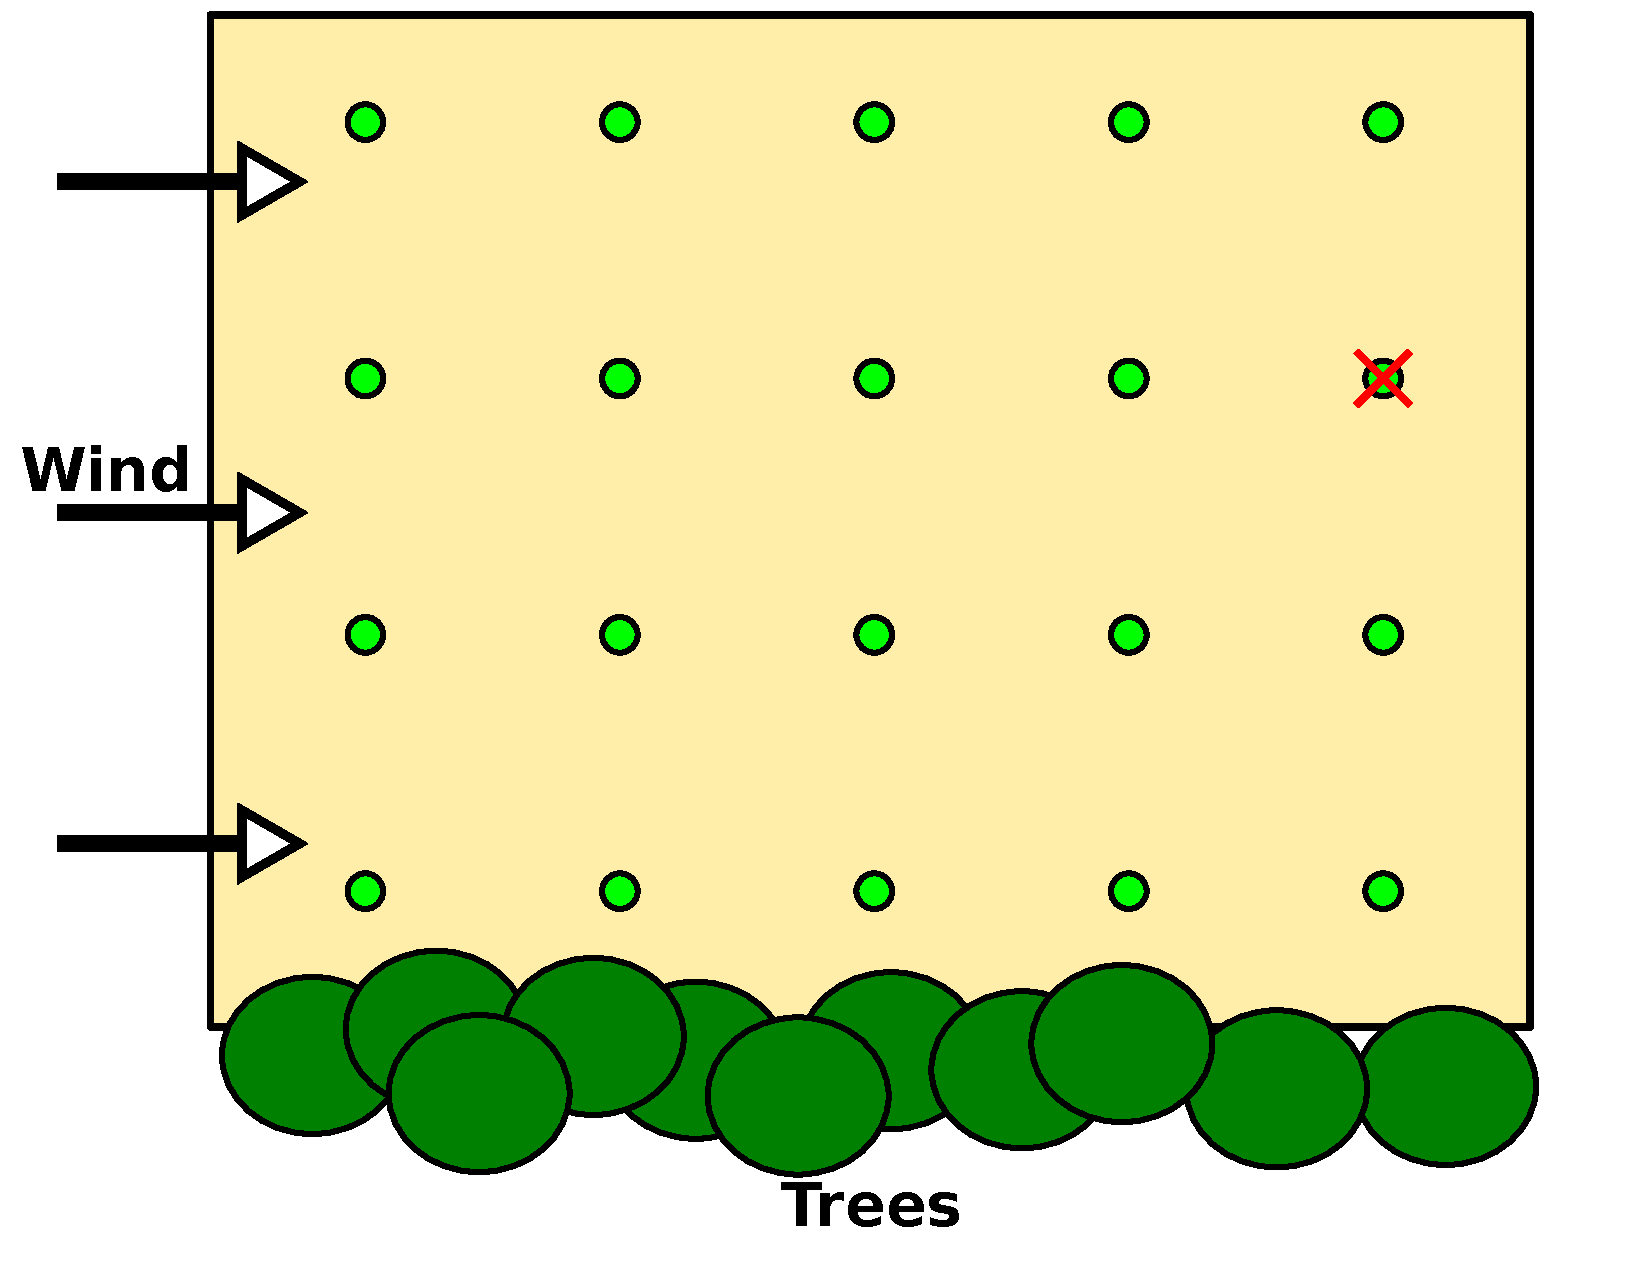
\includegraphics[width=3.0in]{./Figures/field}
\end{center}
\caption{Schematic of experimental field. The green dots are data loggers, and the red X represents a broken device.}
\label{fig:field} 
\end{figure}

Several models will be constructed to estimate the flame spread rate, but first we take an inventory of the available data. From each of the data loggers we have the time at which the flame reached the device. If we consider flame spread in the downwind direction and take only point-to-point observations of the travel time from one device to the next, then the twenty data loggers embeded in a grid on the grass field produce sixteen unique spread rates. Four measurements came from a boundary that could have been affected by nearby trees and will be discarded to focus on grass flame spread. Of the remaining data loggers, one malfunctioned and will also be discarded (Figure~\ref{fig:field}. The result is eleven flame spread rate observations that will be treated as independent assuming that the flame spread rate has reached a quasi-steady state by the time it arrives at the first row of data loggers.

Accompanying each flame spread observation is a preburn moisture content ($M$) measurement of the grass. However, three of these scenario data points are missing, and can be estimated from the surrounding measurements. These will remain as point estimates for the purpose of this exercise, but it should be noted that a full model would include uncertainty information for the missing values. These values could also be discarded, and the effect of this will be examined briefly using the best fitting model.

The parameters $\sigma$, $M_{ext}$, and $h$ do not have any scenario data and while recommended values are provided by the U.S. Forest Service (ref fuel models) there is no uncertainty information. Prior probability density functions will be chosen for each parameter based on the recommended values and compared to diffuse priors. The remaining parameters in Equation~\ref{eq:roth_fun3} ($w_O$, $\delta$, $\rho_p$ and $U$) are irreducable and scenario specific. Unfortunately, these are only available on a field-wide level with limited uncertainty information. Similar to the missing moisture content scenario parameter, a full analysis would include uncertainty models for each of these parameters from field data however they will remain fixed in the following models (see Appendix~\ref{ap:table}).

Previous research was conducted with a higher order physics-based model focused on testing the sensitivity of flame spread rate to multiple input parameters (ref FireTech). The results of this study suggest that flame spread rate is most sensitive to $\sigma$ and $M$. Therefore, these parameters are the QoIs whose effect on the uncertainty of the flame spread rate is a desired output of the following analysis.

We may now begin constructing the statistical model for this problem. The likelihood function for each of the models is assumed to be normally distributed with the form

\begin{equation}
Y_i \sim \mathcal{N}(R_i,\tau^2),\quad i = 1,...,11
\label{eq:like}
\end{equation}

\noindent where $Y_i$ is an observation of the spread rate, $R_i$ is the spread rate calculated from Equation~\ref{eq:roth_fun3}, and the prior distribution for $\tau$ is

\begin{equation}
\tau \sim \mathcal{U}(0,100)
\label{eq:tau_prior}
\end{equation}

We will define four models with different sets of priors on $\sigma$, $M_{ext}$, and $h$. The first model represents the ``uninformed'' case, however we can not use truly uninformed priors because extreme values result in non-physical rates of spread. Likewise, combinations of extreme non-physical inputs can also produce a physical rate of spread. We must then limit each parameter to a wide physically realistic space. The most ``uninformed'' way to accomplish this is to choose wide uniform priors which is common practice for Bayesian modeling of physical thermal and fluid systems (cite turbulence and combustion papers). The priors for Model 1 are chosen as follows:

\begin{align}
\begin{array}{ccc}
M_{ext} &\sim& \mathcal{U}(0,1) \\
\sigma &\sim& \mathcal{U}(500,50000) \\
h &\sim& \mathcal{U}(1,50000)
\end{array}
\label{eq:mod1_priors}
\end{align}

The motivation choosing the following models will be discussed in Section~\ref{sec:res}, and for now we will simply describe their developement. For Model 2, we will illicit prior information on the mean $M_{ext}$ from Scott, et al (cite USFS) and high estimate from ``expert'' opinion. The mean of the $M_{ext}$ values from literature is calculated to be 0.268 and it is estimated that there is a 99\% probability that $M_{ext}$ is less than 0.6. We choose to use a Gamma prior as $M_{ext}$ is a positive value without a clear upper bound. Using this information with the equations for the mean and cumulative distribution function we have two equations and two unknowns and can numerically solve for the parameters $\alpha$ and $\beta$, leading us to the formulation of Model 2.

\begin{align}
\begin{array}{ccc}
M_{ext} &\sim& \Gamma(5.6,20.87) \\
\sigma &\sim& \mathcal{U}(500,50000) \\
h &\sim& \mathcal{U}(1,50000)
\end{array}
\label{eq:mod2_priors}
\end{align}

Model 3 informed SAV and Mext

Model 4 best of 1, 2, and 3 based on DIC without estimated moisture content points.

Note: Heat of combustion not considered for informed prior as only one value given for all models and there are a variety measurement techniques that can give significantly different results for the same type of fuel.

Model code will be provided with the report, but is not necessary to include.


\section{Results and Analysis}
\label{sec:res}

Describe tuning process. Aim for good mixing and low autocorrelation. Choose iterations such that each produces the same number of samples.

Posterior output. Did it fit? Are the values physically significant? What is the uncertainty? What about outliers (check estimated mc data points)? 

Model 1: High uncertainty, possibility of flame spread in very damp grass (MC over .5) is unlikely, suggest need for prior knowledge on Mext leading to model two.

Model 2:

Model 3:

DIC Table

Now we choose Model X and remove the estimated moisture content scenario parameters. This model will be reffered to as Model 4.

Model 4: uncertainty in spread and sav? DIC? Where the estimated point outliers in previous models?

What is the physical interpretation of this uncertainty? (ie maybe do a simple calculation to see the time frame in which fire could spread over a whole field to give a sense of scale, andor make analogy to huricane forecasting bands with 95 percent confidence interval) 

Compare 95 percent posterior intervals of parameters to range tested in the naive sensitivity approach from firetech paper. Compare spread rates (add points to previous figures and make new ones).

There is a great deal of uncertainty with just the simplified model that has fixed parameters/informed priors etc, comment on need for more scenario data to make up for parameters with identifiability issues and need for better models based more on physics and less on correlations.

Conclude with possibility of extension to more complicated forecasting models.

\clearpage
\appendix
\section{Appendix: Rothermal Input Parameters}
\label{ap:table}

\begin{table}[h]
\caption{PARAMETERS}
\begin{center}
  \begin{tabular}{cccc}
    \hline\noalign{\smallskip}
    Parameter & Symbol & Value & Units \\
    \noalign{\smallskip}\hline\noalign{\smallskip}
    Front (Flame) Side Temperature & $T_\infty$ & $K$\\
    Flame Side Heat Transfer Coefficient & $h$ & $\frac{W}{m^2K}$\\ 
    Material Specific Heat & $c$ & $\frac{J}{kgK}$\\ 
    Material Conductivity & $k$ & $\frac{W}{mK}$\\ 
    Back Side Gas Temperature & $T_{\infty,b}$ & $K$\\ 
    Back Side Heat Transfer Coefficient & $h_b$ & $\frac{W}{m^2K}$\\ 
    \noalign{\smallskip}\hline
  \end{tabular}
\end{center}
\label{tab:para}
\end{table}

\section{Appendix: PyMC Model Code}

% \bibliographystyle{unsrt}
% \bibliography{./flameBayesBiblio}

\end{document}
